\documentclass[twotcolumn]{scndocument}

\newcommand{\RNumb}[1]{\uppercase\expandafter{\romannumeral #1\relax}}
\usepackage{multicol}
\usepackage{lipsum}
\usepackage{tikz}
\usepackage{float}
\usepackage{graphicx}
\usepackage[usenames]{hyperref}
\begin{document}
\begin{multicols}{2}
key advantage that other methods lacked: preserving the
privacy of images.
\par Data leakage does not occur because clients only
exchange a portion of the weights with the server, which
is insufficient to reconstruct the original data on which
the model was trained.
\par It is precisely this advantage that enables the use of this
algorithm for training models used for medical images,
ensuring the privacy and confidentiality of sensitive
patient data.
\par Among the drawbacks of this approach, the following
can be identified: \begin{itemize}
\item The need for additional training of the server model:
This requires extra time and additional data for
training the server model.
\item Lack of improvement in model quality when the
number of weights transmitted by clients for aggregation is too small: If the amount of weight
information shared by clients is insufficient, the
overall model quality may not improve significantly.
\item Potential degradation in model quality when the
architectures of the models differ significantly: If
the models used by the clients have vastly different
architectures, the aggregation process may lead to a
decrease in model quality instead of improvement. \end{itemize}
\vspace{3mm} \begin{center}
\RNumb{5}. Experiments and Results
\end{center} \vspace{2mm}
\par For the analysis of the effectiveness of the developed
method, a dataset of 12,000 histological images was
used, divided into two classes: malignant tumors and
benign tumors. The dataset consisted of 8,400 images
for training and 3,600 images for testing. The training
dataset was randomly divided into five parts: four clients
and one server.
\par The training process involved a cycle of weight exchange between the clients and the server, followed by
aggregation and sending back of the weights. This cycle
was performed every 3 epochs of training, and a total of
10 cycles were conducted.
\par The weights for aggregation
were sent from each client. Therefore, the total number
of training epochs for each client was 30.
The weights of the models for exchange (Rk space)
were the weight matrices of the linear classification layer
of the network, with a dimension of 1024x1024 for all
clients.
\par The evaluation of the method was done by comparing
the following values obtained with and without the
application of this method during training (traditional
training without weight aggregation for 30 epochs): \begin{itemize}
\item The meaning of the loss function (cross-entropy)
during training.
\item The value of the loss function on the test dataset.
\item The accuracy of predictions on the test dataset. \end{itemize} \columnbreak
 \textit{ A. Models with the same architecture} \vspace{1mm}
\par For analyzing the effectiveness of the developed
method in the case of homogeneity of local models, was
used a simple neural network with the architecture shown
\href{https://proc.ostis.net/proc/Proceedings%20OSTIS-2024.pdf}{\textcolor{blue}{2}}: \par
\begin{figure}[H]
  \centering
    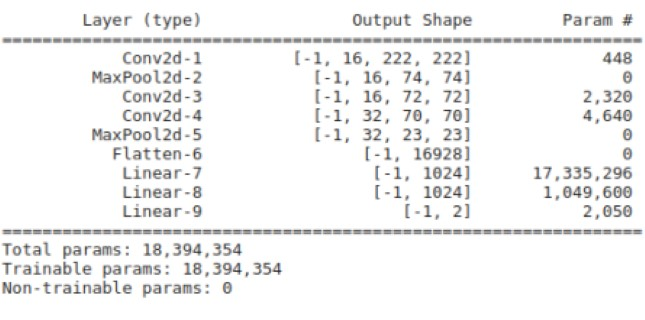
\includegraphics[width=8cm,height=4cm]{image.png}
  \caption{Simple neural network architecture.}
\end{figure}
\par As the global model (server), a pre-trained resnet18
network was used, fine-tuned on 1170 histological images
for 30 epochs. For weight aggregation from clients, the
last layer designed for classification was modified to the
following:
\par For weight aggregation, a linear layer called "aggregate" is used. It takes weights from clients as input
for aggregation and produces modified weights for each
client as output.
\par In the figure \textcolor{blue}{4} is a graph showing the evaluation of
various quality metrics for client 0 (the graphs for other
clients are similar).
\par Based on the analyzed data graphs, the following
conclusions can be drawn about the performance of this
method on simple models of the same architecture: \begin{itemize}
\item For all clients, there is a decrease and stability in
the values of the loss function during training when
the method is applied.
• For 3/4 of the clients, there is higher stability in the
accuracy of predictions on the test dataset when the
method is applied.
\item The average prediction accuracy did not change
when the method was applied. \end{itemize}
\vspace{2mm} \textit{B. Models of various architectures} \vspace{1mm}
\par The following pretrained neural networks were used to
analyze the effectiveness in the case of heterogeneity of
local models: \begin{itemize}
\item Client 1: SimpleModel (see above);
\item Client 2: MobileNetV3 Large;
\item Client 3: MobileNetV3 Small;
\item Client 4: DenseNet121. \end{itemize}
\par For each local model, the last layer of the neural network was replaced with the layer shown in the figure \textcolor{blue}{5}:
\par The transferred weights are the weights of the shared
linear layer. The model for the server is similar to the
model from the previous section.
\end{multicols}{ }
\begin{figure}[H]
  \centering
    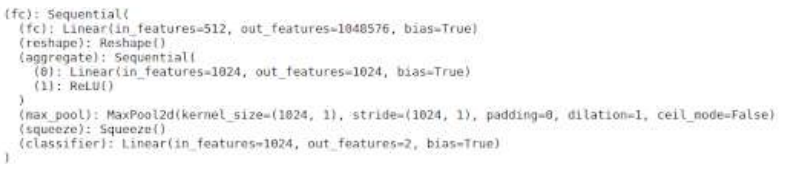
\includegraphics[width=17cm,height=4cm]{image2.png}
  \caption{The last layer of the resnet18 network for weight aggregation.}
\end{figure} 
\begin{figure}[H]
  \centering
    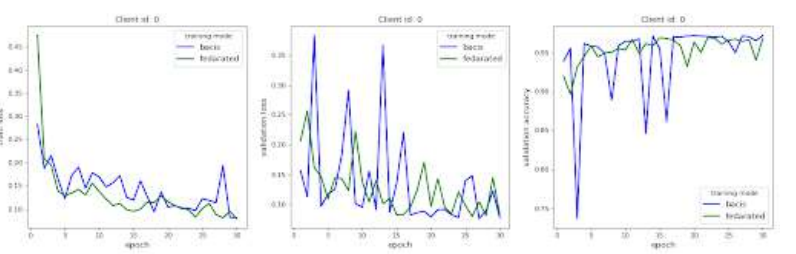
\includegraphics[width=17cm,height=5cm]{image3.png}
  \caption{Graphs of analyzed metrics (SimpleModel).}
\end{figure} 
\begin{figure}[H]
  \centering
    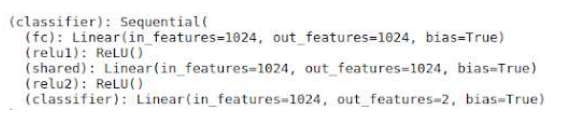
\includegraphics[width=12cm,height=2.5cm]{image4.png}
  \caption{The last layer of the local models.}
\end{figure}
\begin{multicols}{2}
\par In figures \textcolor{blue}{6} and \textcolor{blue}{7} are the plots showing the evaluation
of various quality metrics for clients 0 and 2.
\par Based on the analyzed data graphs, the following
conclusions can be drawn about the performance of this
method on pre-trained models of various architectures: \begin{itemize} \vspace{-1mm}
\item \vspace{-1mm} For all clients, there is a decrease and stability in
the values of the loss function during training when
the method is applied.
\item There is higher stability in the prediction accuracy
on the test dataset for simpler models and some pretrained networks when the method is applied. 
\item \vspace{-1mm} On average, the prediction accuracy with the method
applied has not changed. \end{itemize} 
\textit{C. Heterogeneous data}
\par In real life, it is possible for data to be stored on different media. Additionally, the data can be heterogeneous.
\par To analyze the effectiveness in the case of data heterogeneity, consider a scenario where the original dataset
is divided into two clients. The data of the first client
contains 95 of class 0 objects and 5% of class 1 objects.
Conversely, the second client has 5% of class 0 objects
and 95 of class 1 objects.
\columnbreak
\par Architecture of client models
is shown below
\par As the global model a pre-trained resnet18 network
was used. For weight aggregation from clients, the last
layer designed for classification was modified to the layer
in the figure \textcolor{blue}{9}
\par During the training process of the second and third
models, federated learning was used. The FedAVG algorithm was selected for aggregating information from
client models.
\par The exchange of model weights between the client
models and the server occurred every 3 epochs. Each
of the client models was trained for a total of 30 epochs.
The cross-entropy loss function was used.
\par The goal of the experiment was to study the dependence of model prediction accuracy on the partitioning
of the dataset among clients.
\par Thus, we simulate a situation where the data from
different clients is highly heterogeneous
\par In such a situation, it is not possible to achieve
\end{multicols}
\begin{figure}[H]
  \centering
    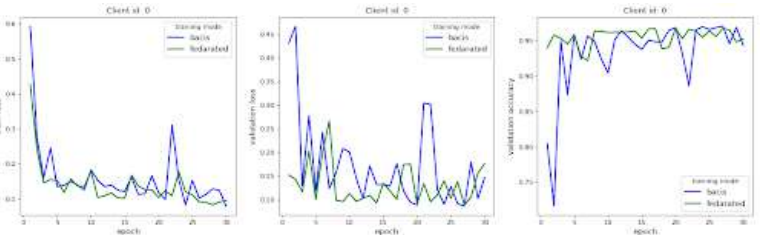
\includegraphics[width=17cm,height=5cm]{image5.png}
  \caption{ Graphs of analyzed metrics (SimpleModel).}
\end{figure} 
\begin{figure}[H]
  \centering
    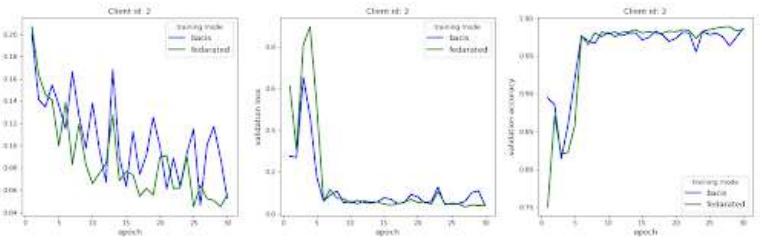
\includegraphics[width=17cm,height=5cm]{image6.png}
  \caption{Graphs of analyzed metrics (MobileNetV3 Large).}
\end{figure} 
\begin{figure}[H]
  \centering
    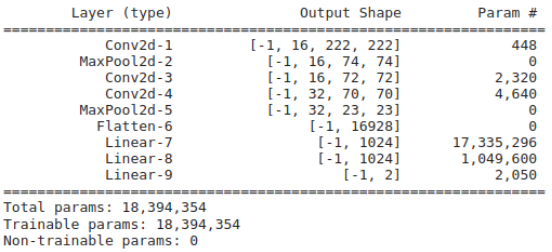
\includegraphics[width=12cm,height=6cm]{image7.png}
  \caption{Client model architecture.}
\end{figure} 
\begin{figure}[H]
  \centering
    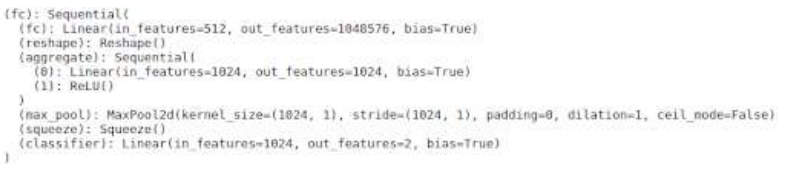
\includegraphics[width=16cm,height=4cm]{image8.png}
  \caption{The last layer of the resnet18 network for weight aggregation.}
\end{figure} 
\end{document}
